\documentclass[aps,onecolumn,twoside,secnumarabic,balancelastpage,amsmath,amssymb,nofootinbib,hyperref=pdftex]{revtex4}


\usepackage{color}         % produces boxes or entire pages with colored backgrounds
\usepackage{multirow}
\usepackage{graphics}      % standard graphics specifications
\usepackage[pdftex]{graphicx}      % alternative graphics specifications
\usepackage{longtable}     % helps with long table options
\usepackage[english]{babel}
\setlength{\parskip}{1em}
\usepackage{amsmath}
\usepackage{epsf}          % old package handles encapsulated post script issues
\usepackage{bm}            % special 'bold-math' package
\usepackage{verbatim}			% for comment environment
\usepackage[colorlinks=true]{hyperref}  % this package should be added after all others % use as follows: \url{http://web.mit.edu/8.13}                                    
                                  

\begin{document}
\title{Dark Photons at the ILC}
\author         {Noah Steinberg}
\email          {nastein@umich.edu}
\date{\today}
\affiliation{University of Michigan - Physics}

\maketitle

\section {Massive dark photon lagrangian}

We would like to study the phenomenology of a massive dark photon $A^{'\mu}$ with the following lagrangian
\begin{equation}
\mathcal{L} = \mathcal{L_{\text{SM}}} - \frac{1}{4}\tilde{F}'^{\mu\nu}\tilde{F}'_{\mu\nu} + \frac{\varepsilon}{2cos\theta_{W}}B_{\mu\nu}\tilde{F}'^{\mu\nu} - \frac{m'^{2}}{2}\tilde{A}'^{\mu}\tilde{A}'_{\mu},
\end{equation}
where $B_{\mu\nu}$ is the U(1) hypercharge field strength and $\tilde{A}'^{\mu}$ is the dark photon with lagrangian mass $m'$, and field strength $\tilde{F}'^{\mu\nu}$. We have chosen the normalization of the hypercharge/dark photon mixing so that after diaganolization into mass eigenstates ($Z_{\mu}, A_{\mu}, A'_{\mu}$), the coupling of the mass eigenstate $A'^{\mu}$ to the standard model EM current is
\begin{equation}
\mathcal{L} \supset -e\varepsilon J^{\mu}A'_{\mu}.
\end{equation}
We see that the dark photon couples to the standard model EM current with coupling strength $\varepsilon e$\footnote{The Z boson and photon also couple to the dark current, but these couplings will not effect the phenemonology we discuss here}.

\section{Dark photon branching ratios}
For a generic dark sector, computing the dark photon branching ratios is impossible because of the sector's unknown particle content. Simplifications occur if we consider a dark sector with other particles, generically denoted by $\chi$, with masses satisfying $m' < 2m_{\chi}$. Then the dark photon can only decay to visible SM particles and computing the dark photon branching ratios is a relatively straightforward calculation, depending only on the parameter space ($m'$,$\varepsilon$).
\vskip 0.12in
The decay width of the massive dark photon into SM fermion pairs $f\bar{f}$ is given by
\begin{equation}
\Gamma(A' \rightarrow f\bar{f}) = N_{c}Q^{2}\frac{1}{3}\alpha\varepsilon^{2}m'\sqrt{1 - \frac{4m_{f}^{2}}{m'^{2}}}(1 + \frac{2m_{f}^{2}}{m'^{2}}),
\end{equation}
where $N_{c} = 3(1)$ for quarks(leptons), and $Q$ is the electric charge of the fermion in units of the fundamental charge, $e$. This formula is good for $m' > 2$ GeV where perturbative QCD is valid. This can be noted by examining $R(s) = \sigma_{e^{+}e^{-}\rightarrow had}/\sigma_{e^{+}e^{-}\rightarrow \mu^{+}\mu^{-}}$, which matches with perturbative QCD above $\sqrt{s} = 2 GeV$. At energies below 2 GeV, there are nonperturbative threshold effects and resonances which modify the formula. But for $\varepsilon \ll 1$ the coupling of the dark photon to SM fermions is photon like, so at masses below 2 GeV one can approximate to high precision the partial widths of the dark photon via the formula
\begin{equation}
\Gamma(A' \rightarrow \text{hadrons}) = \frac{1}{3}\alpha\varepsilon^{2}m'\sqrt{1 - \frac{4m_{\mu}^{2}}{m'^{2}}}(1 + \frac{2m_{\mu}^{2}}{m'^{2}})R(\sqrt{s} = m').
\end{equation}
Thus for a range of interesting masses above 1 MeV, the dark photon branching ratios can be computed using the above formulas. We utilize the DarkCast software to compute the dark photon branching ratios for masses from 100 MeV to 10 GeV. DarkCast utilizes worldwide data on $e^{+}e^{-}\rightarrow\text{hadrons}$ cross sections over a range of center of mass energies. Above 2 GeV, perturbative QCD is used once again and no resonances are included. Below in Fig.~\ref{fig:BR} we plot the branching ratios of an $A'_{\mu}$ into pairs of electrons, muons, taus, light hadrons\footnote{These are hadrons containing the light quarks u,d,s}, charm and bottom quarks. One can see between 100 MeV and 2 GeV the resonances from light hadrons, and the gradual turning on of the heavier quarks as $m'$ increases. Decays into pairs of electrons, muons, and taus all have the same branching ratio ($\text{BR}_{l\bar{l}}\approx .15$) when $m' > 8$ GeV.
\begin{figure}[htbp]
\begin{center}
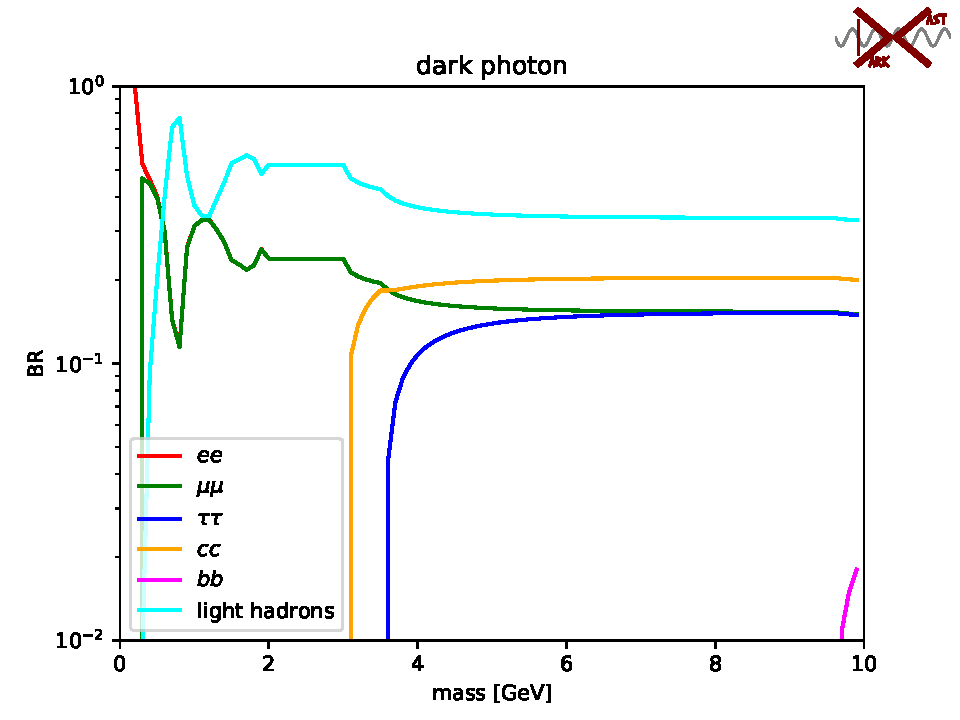
\includegraphics[width=12cm]{BR.pdf}
\caption{default}
\label{fig:BR}
\end{center}
\end{figure}




















\end{document}